
\section{State of the Art}\label{SOTA}
Def: State of the art
\textit{ State of the art is the level of knowledge and development achieved in a technique, science, etc, esp at present }
\newline
This section will be an analysis of a number of applications that all focus on designing a room or a set of rooms and the navigation in them. The previous sections have provided the necessary framework for doing the analysis. Specifically the analysis will cover:

\begin{itemize}
\item The familiarity of the different aspects of the apps.\\
What parts of the app have been seen in other apps or in real life. 
\item The knowledge space for the app\\
Here the analysis will try to determine if the app succesfully bridges the knowledge gap talked about in ux section ref: fig. \ref{fig:Knowledge}.
\item The graphical design\\
Colours and layout.
\item The different interaction methods that are used. 
\end{itemize}
 Finally the end of this section will sum up the trends noted and will give an overview of what aspects the different applications have lacked behind with and what aspects this project could aim to improve. 

\subsection{Ikea Kitchen Planner}
In this application customers can create accurate measurements of their own kitchen and place the furniture from IKEA's catalogue. It is possible to do different wall measurements, add wallpapers to walls, apply different ceiling and floor covers, add windows and doors. Users can view the layout from top-down view and later see how the furnished layout looks in 3D perspective.

IKEA's web application for designing kitchens is used mainly in actual IKEA stores. This could indicate that users need help using this application It is used as a tool with focus on efficiency and not so much an app you would use at home for interior design.

When you first enter the app there is no immediate help or tutorial. There is, however, two places in the app where it is possible to get help yourself. Very reasonable layout going from left to right and top to bottom. There is a lot of easily recognizable buttons which help the user experience along. 
It is very slow though which highly affects the usability. The app uses click and drag.

\begin{figure}[H]
\centering
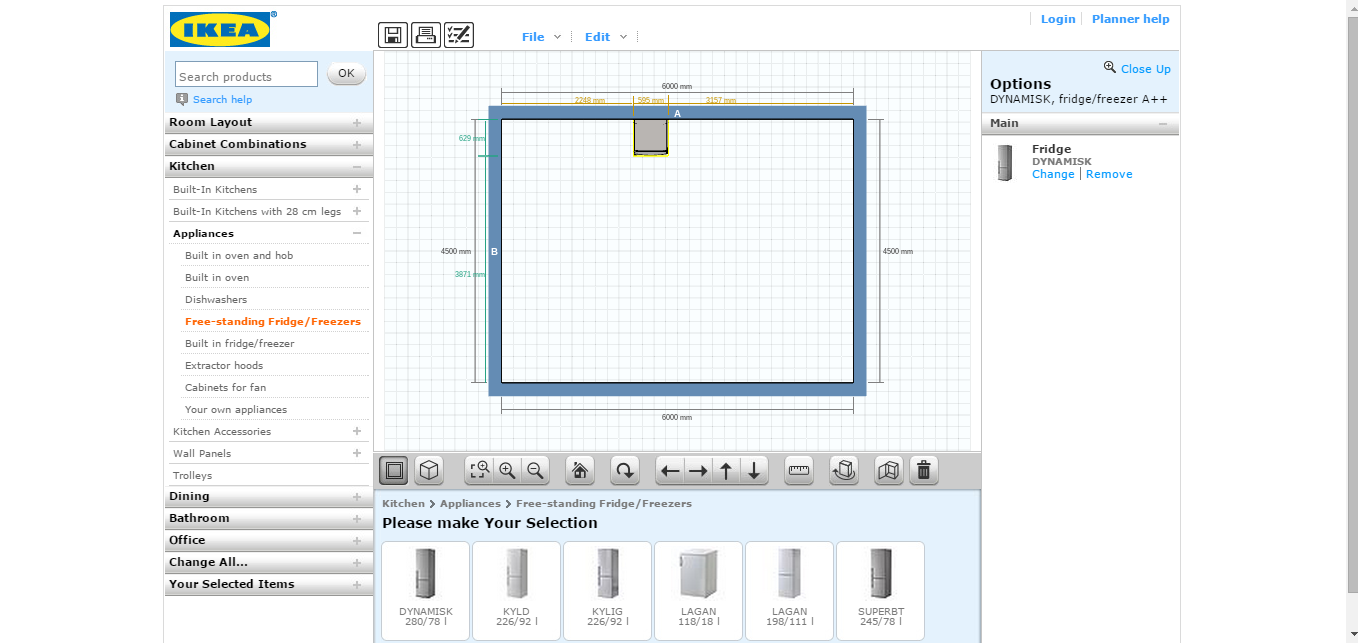
\includegraphics[scale=0.25]{IKEAPlanner.png}
\caption{IKEAs kitchen planner webapplication in 2D mode.}
\end{figure}

The app is grey and clinical but again, it is a practical tool for IKEA customers to visualize a kitchen. 
The application offers plenty of useful features and can be used to give a grasp of how peoples homes would look like prior to buying the actual items, however, it is rarely used by IKEA's customers. The problem could be that the application is hard to use, leading to long time spans used to build the desired kitchen design. A solution to this possible problem could be to create an application that is more intuitive and takes less time to achieve the users needs.

\subsection{HomeDesign3D}
This mobile application is made for interior design. It has most of the basic features; building rooms, placing furniture, windows and doors. The user can then switch to a 3D view. There are two control schemes to choose from - a joystick where you use both thumbs to move around the house, or arrows where you can view the room by moving your finger around and use the arrows to move from room to room. From the 3D view you can paint the walls and change the flooring.

\begin{figure}[H]
\centering
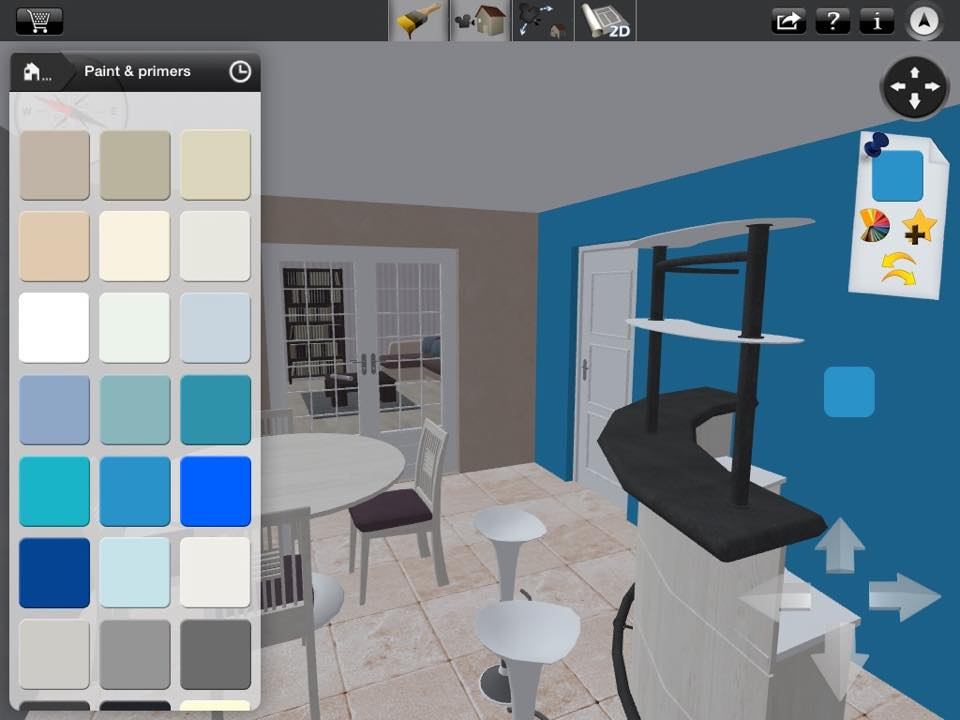
\includegraphics[scale=0.25]{HomeDesign3D.jpg}
\caption{HomeDesign3D application. Painting walls.}
\end{figure}

When you first enter the app you are faced with the option of buying the full version. This is actually the start of a long tutorial. It is very hard to notice though, since the points at the bottom that indicates that you can swipe is covered by a commercial. It is very unlikely that the user will find this help from the beginning and therefore will properly “go back” to the menu. The tutorial is easy to understand but very long. It has both pictures and text. It looks messy because of the background and the hand drawn hand that shows how to do the different things. It is not very consistent in matters of graphical design. 

The next step is the design. There is apparently no start menu or the likes. 
The icons are easy recognizable.  

The layout looks very cluttered. There is a big commercial at the bottom and the menu bar in the top. 
The mix of the black bars and buttons with the beige background does not go very well together. The fact that the background is textured as a wall as well does not help the graphical aspect of this app. 

\subsection{AutoDesks HomeStyler}
This app is Autodesk's attempt at making an interior design app. The app does not provide a user guide from when you open up the app, this is opposed to the idea about bridging the knowledge gap with tutorials. The app does however provide a guide for users, once they are actually designing their room but if the user is not able to get to this point then they are stuck. The overall look of the app is reminiscent of the flat design pattern as seen in Windows 8, this makes the app look very exclusive. However during the main activity of the app the design does not exactly match the look when browsing the catalogue, this leads to the app lacking consistency. 

\begin{figure}[H]
\centering
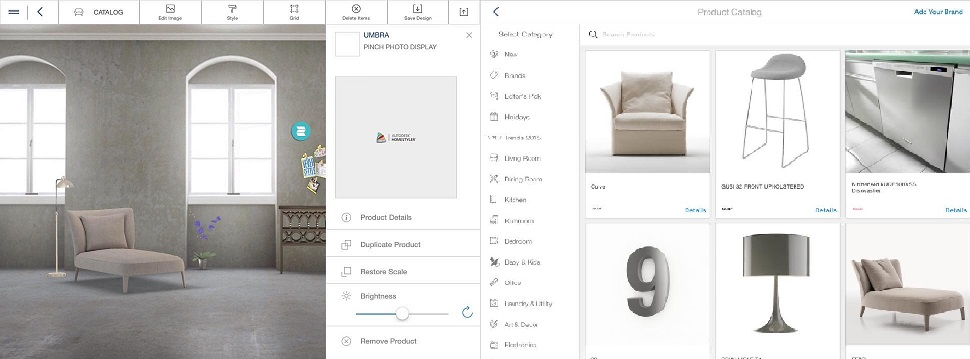
\includegraphics[scale=0.50]{AutodeskCombined.jpg}
\caption{Homestyler's lack of consistency. Right: The design of the catalogue. Left: The design of the actual room planning feature.}
\end{figure}

The app's button design also seems to be focused on bigger screens than a smartphone. The 
big button at the top, labeled "Redesign" is a good example of both the isolation effect mentioned in section \ref{isolationFig} and also the button follows the principle of having the buttons be labeled with a single word 
(section \ref{DesigningIntuitively}). The interaction in the app is primarily clicks with some multi touch functions for the more advanced functions such as resizing, moving, rotating furniture. These functions are explained the first time the user is using them and then never again.

\subsection{State of the Art Conclusion}

To sum up, the applications use a variety of controls. Most of them use click and drag, some a bit of multi touch and one has two options; joystick or buttons. 
In general the apps seem to have a different focus, therefore a different outcome.

What we can conclude from this, is that two in three use non-traditional interaction to their advance. Only one has a tutorial tha;t is not text based and provides the optimal knowledge at the first encounter or makes the user interface so intuitive or familiar that a tutorial is unnecessary.
